\chapter{Conceptos Fundamentales}

\section{Puntos de Equilibrio}

En el estudio de sistemas dinámicos, los \textbf{puntos de equilibrio} desempeñan un papel fundamental como estados en los que las variables del sistema permanecen constantes. Formalmente, para un sistema lineal en el plano de la forma 
\[
\frac{d\mathbf{x}}{dt} = A\mathbf{x}, \quad \text{donde } \mathbf{x} = \begin{bmatrix} x \\ y \end{bmatrix} \text{ y } A \text{ es una matriz } 2 \times 2,
\]
un punto $\mathbf{x}_0$ es un punto de equilibrio si satisface $A\mathbf{x}_0 = 0$. Estos puntos representan estados estacionarios del sistema, y su clasificación nos permite entender el comportamiento global del sistema dinámico.

En esta sección, exploraremos los diferentes tipos de puntos de equilibrio que pueden surgir en sistemas lineales, enfocándonos en su clasificación según los valores propios (eigenvalores) de la matriz $A$. Además, analizaremos sus implicaciones geométricas y dinámicas, proporcionando ejemplos concretos para ilustrar cada caso.

\subsection{Puntos de Equilibrio Robustos a Perturbaciones}

Los puntos de equilibrio robustos son aquellos cuyo comportamiento cualitativo permanece inalterado bajo pequeñas perturbaciones en el sistema. Esta robustez los hace particularmente interesantes desde el punto de vista de la estabilidad y la predictibilidad.

\subsubsection{Nodos}

\begin{definition}
Un \textbf{nodo} ocurre cuando los eigenvalores $\lambda_1$ y $\lambda_2$ de la matriz $A$ son reales y tienen el mismo signo. Si ambos son negativos, el nodo es estable; si ambos son positivos, es inestable.
\end{definition}

En un nodo, las trayectorias convergen o divergen hacia el origen dependiendo del signo de los eigenvalores. Las soluciones tienden a alinearse con la dirección asociada al eigenvalor de mayor magnitud, conocida como la "dirección más rápida". Esta propiedad refleja cómo el sistema prioriza ciertas direcciones en su evolución temporal.

\begin{example}
Consideremos el sistema:
\[
\frac{d}{dt} \begin{bmatrix} x \\ y \end{bmatrix} = \begin{bmatrix} -2 & 0 \\ 0 & -1 \end{bmatrix} \begin{bmatrix} x \\ y \end{bmatrix}.
\]
Los eigenvalores son $\lambda_1 = -2$ y $\lambda_2 = -1$, ambos negativos. Este es un \textbf{nodo estable}. Geométricamente, todas las trayectorias convergen hacia el origen, siendo la dirección del eje $x$ la más rápida debido al mayor valor absoluto de $\lambda_1$.
\end{example}

\begin{figure}[h]
    \centering
    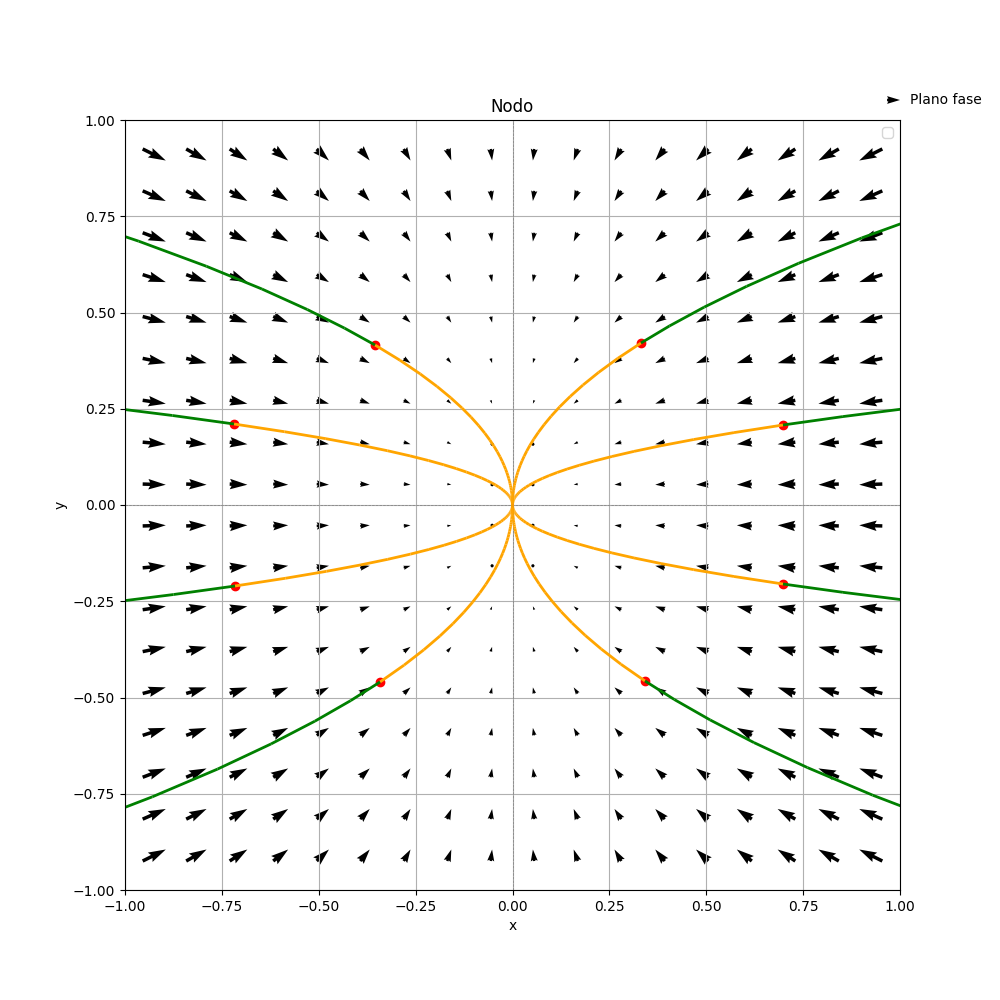
\includegraphics[width=0.7\textwidth]{Img/Nodo.png}
    \caption{Nodo estable}
    \label{fig:nodo}
\end{figure}

El término "nodo" sugiere un punto central al que todas las trayectorias convergen o desde el cual divergen, similar a cómo los nodos en una red conectan múltiples caminos. Esta analogía resulta útil para visualizar el comportamiento de estos sistemas.

\subsubsection{Punto Silla}

\begin{definition}
Un \textbf{punto silla} ocurre cuando los eigenvalores $\lambda_1$ y $\lambda_2$ son reales y tienen signos opuestos ($\lambda_1 > 0$ y $\lambda_2 < 0$).
\end{definition}

El nombre "punto silla" proviene de la analogía con una silla de montar, donde hay direcciones estables (las patas de la silla) y direcciones inestables (el respaldo). Las trayectorias se acercan inicialmente siguiendo la dirección del eigenvalor negativo y luego divergen siguiendo la dirección del eigenvalor positivo.

\begin{example}
Considere el sistema:
\[
\frac{d}{dt} \begin{bmatrix} x \\ y \end{bmatrix} = \begin{bmatrix} 1 & 0 \\ 0 & -1 \end{bmatrix} \begin{bmatrix} x \\ y \end{bmatrix}.
\]
Los eigenvalores son $\lambda_1 = 1$ y $\lambda_2 = -1$. Este es un \textbf{punto silla}. Las trayectorias se comportan como líneas hiperbólicas que convergen hacia el origen en una dirección y divergen en otra.
\end{example}

\begin{figure}[h]
    \centering
    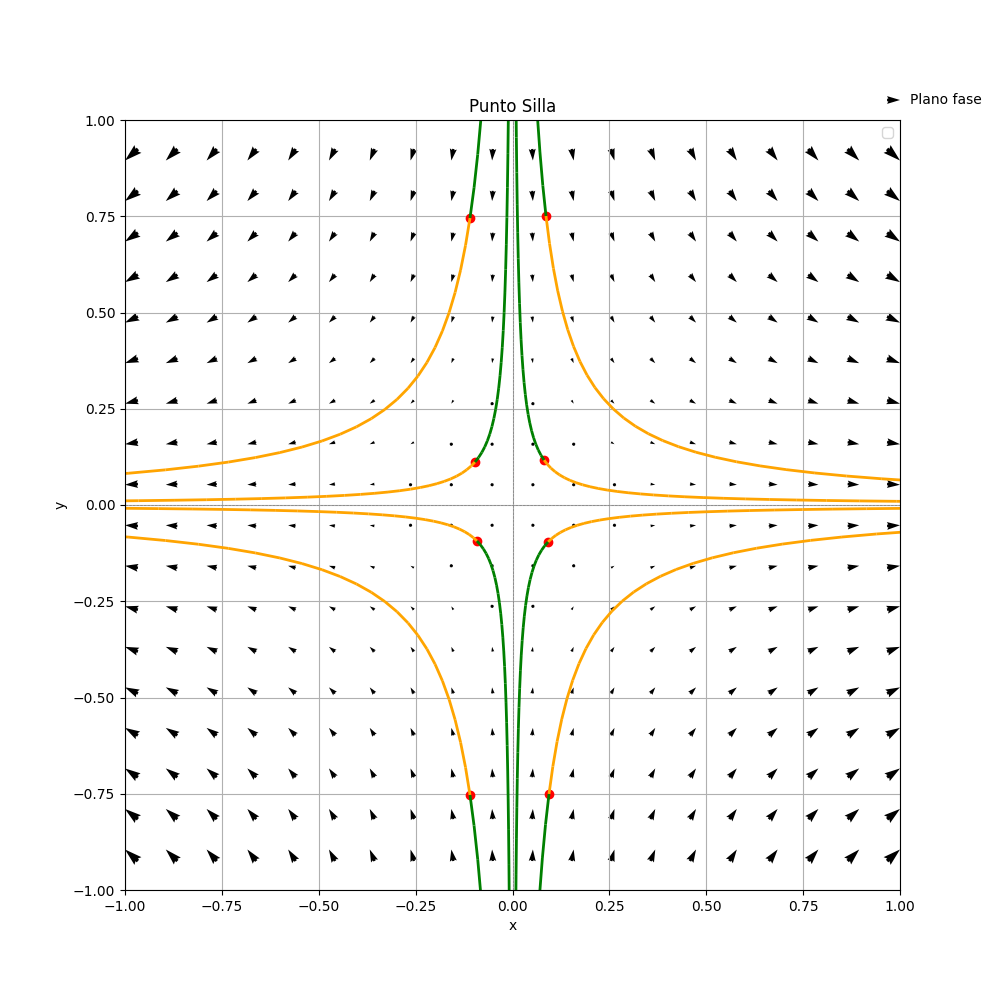
\includegraphics[width=0.7\textwidth]{Img/PuntoSilla.png}
    \caption{Punto silla}
    \label{fig:punto_silla}
\end{figure}

El punto silla es único entre los puntos de equilibrio robustos porque no es ni completamente estable ni completamente inestable. Este comportamiento dual lo convierte en un objeto de estudio fascinante en sistemas dinámicos.

\subsubsection{Espirales}

\begin{definition}
Un \textbf{espiral} ocurre cuando los eigenvalores $\lambda_1$ y $\lambda_2$ son complejos conjugados con parte real distinta de cero. Si la parte real es negativa, el espiral es estable; si es positiva, es inestable.
\end{definition}

En un espiral, las trayectorias giran alrededor del origen mientras convergen o divergen. La frecuencia de rotación está determinada por la parte imaginaria de los eigenvalores, mientras que la parte real dicta la estabilidad o inestabilidad del sistema.

\begin{figure}[h]
    \centering
    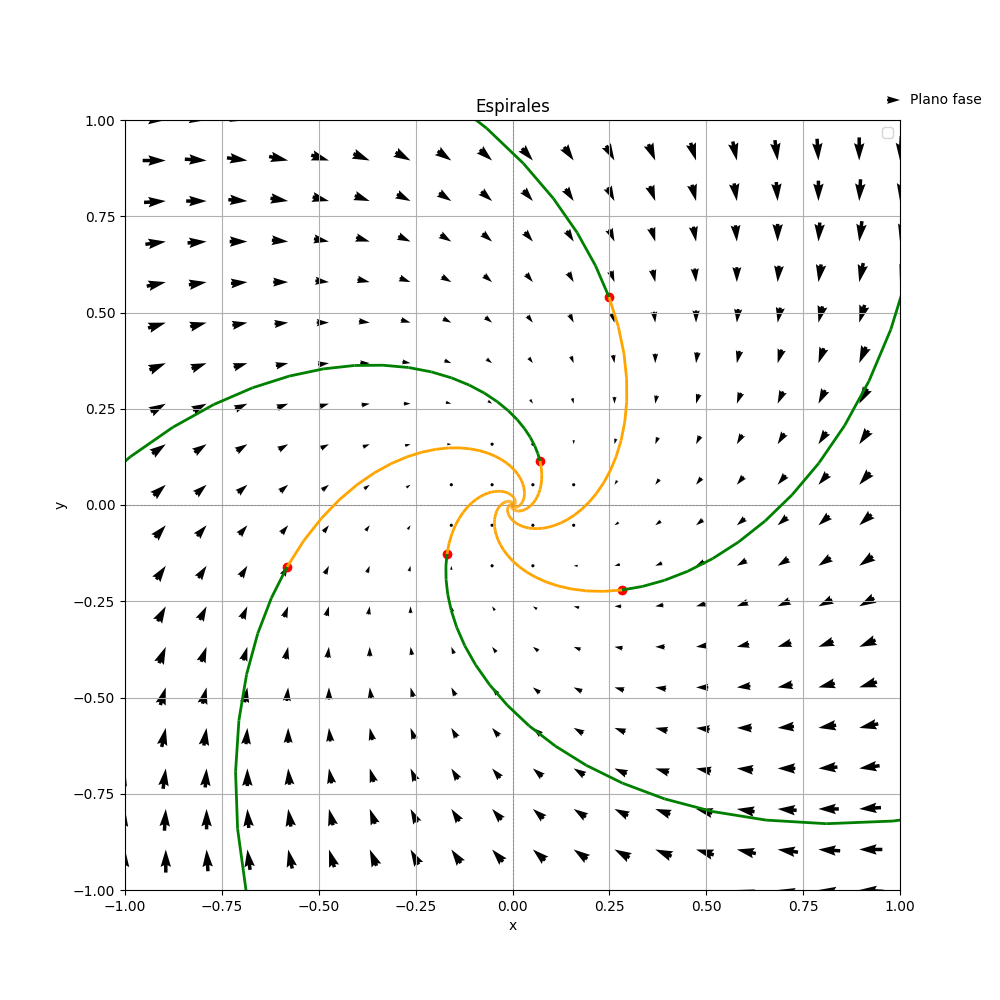
\includegraphics[width=0.7\textwidth]{Img/Espirales.png}
    \caption{Espiral estable}
    \label{fig:espiral}
\end{figure}

\begin{example}
Considere el sistema:
\[
\frac{d}{dt} \begin{bmatrix} x \\ y \end{bmatrix} = \begin{bmatrix} -1 & 1 \\ -1 & -1 \end{bmatrix} \begin{bmatrix} x \\ y \end{bmatrix}.
\]
Los eigenvalores son $\lambda_{1,2} = -1 \pm i$. Este es un \textbf{espiral estable}. Las trayectorias forman espirales que convergen hacia el origen.
\end{example}

La belleza de los espirales radica en su naturaleza dual: combinan rotación y convergencia/divergencia en un solo movimiento. Esto los hace especialmente útiles para modelar fenómenos oscilatorios amortiguados, como un péndulo con fricción.

\subsection{Puntos de Equilibrio Frágiles}

Los puntos de equilibrio frágiles son aquellos cuyo comportamiento puede cambiar drásticamente bajo pequeñas perturbaciones. Estos casos son menos comunes pero igualmente importantes para comprender la estructura de los sistemas dinámicos.

\subsubsection{Nodo Estrella}

\begin{figure}[h]
    \centering
    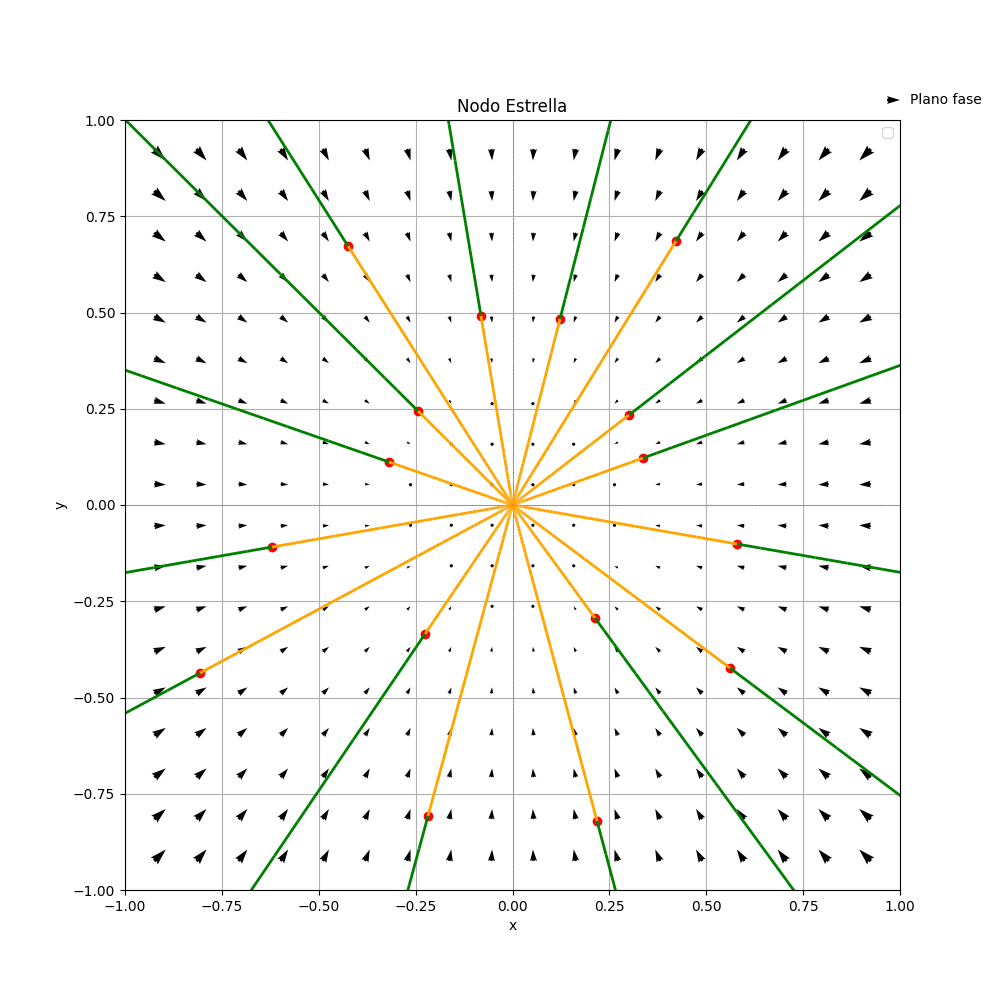
\includegraphics[width=0.7\textwidth]{Img/NodoEstrella.png}
    \caption{Nodo estrella estable}
    \label{fig:nodo_estrella}
\end{figure}

\begin{definition}
Un \textbf{nodo estrella} ocurre cuando los eigenvalores $\lambda_1$ y $\lambda_2$ son iguales y distintos de cero. En este caso, todo $\mathbb{R}^2$ es espacio propio.
\end{definition}

En un nodo estrella, las trayectorias convergen o divergen radialmente desde el origen. Es estable si $\lambda < 0$ e inestable si $\lambda > 0$.

\begin{example}
Considere el sistema:
\[
\frac{d}{dt} \begin{bmatrix} x \\ y \end{bmatrix} = \begin{bmatrix} -1 & 0 \\ 0 & -1 \end{bmatrix} \begin{bmatrix} x \\ y \end{bmatrix}.
\]
Este es un \textbf{nodo estrella estable}. Todas las trayectorias convergen radialmente hacia el origen.
\end{example}

\subsubsection{Nodo Degenerado}

\begin{definition}
Un \textbf{nodo degenerado} ocurre cuando solo existe un vector propio asociado a un único eigenvalor.
\end{definition}

\begin{figure}[h]
    \centering
    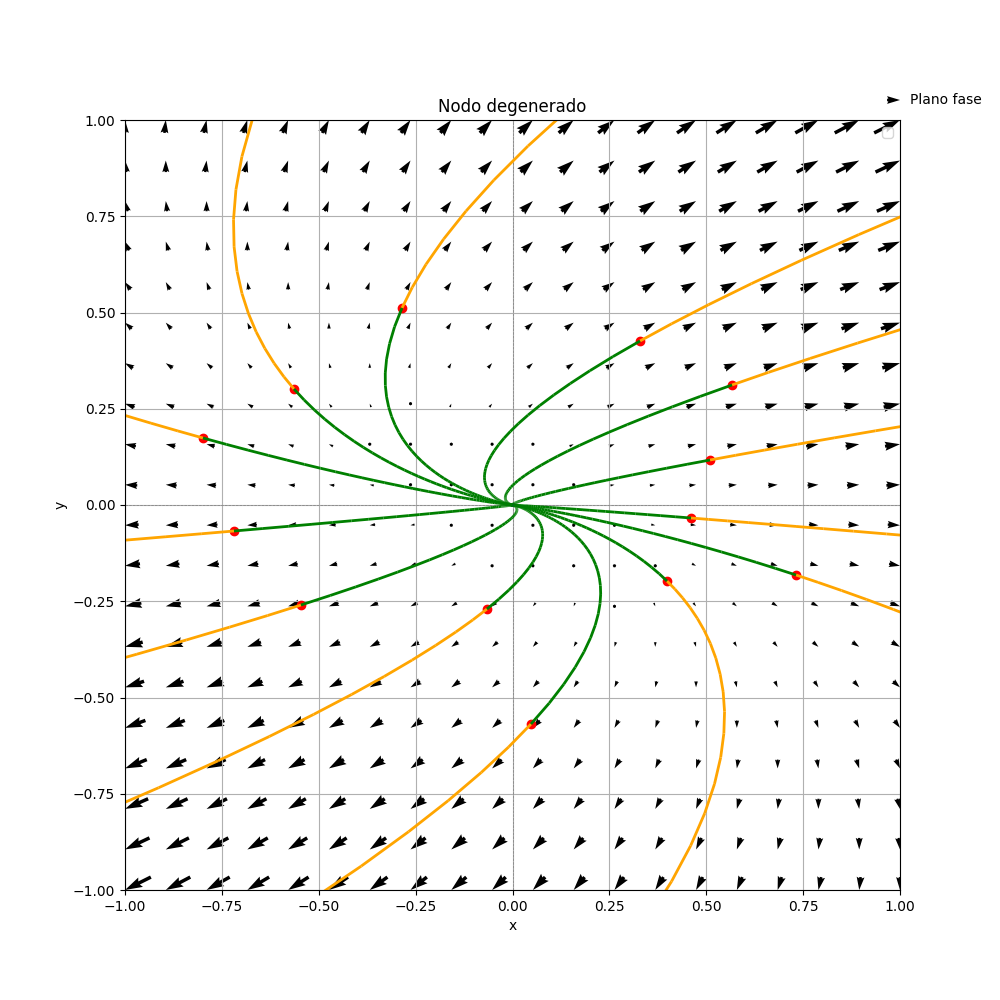
\includegraphics[width=0.7\textwidth]{Img/NodoDegenerado.png}
    \caption{Nodo degenerado inestable}
    \label{fig:nodo_degenerado}
\end{figure}

En un nodo degenerado, las trayectorias convergen o divergen tangencialmente al único vector propio. Es estable si el eigenvalor es negativo e inestable si es positivo.

\begin{example}
Considere el sistema:
\[
\frac{d}{dt} \begin{bmatrix} x \\ y \end{bmatrix} = \begin{bmatrix} 1 & 1 \\ 0 & 1 \end{bmatrix} \begin{bmatrix} x \\ y \end{bmatrix}.
\]
Este es un \textbf{nodo degenerado inestable}.
\end{example}

El nodo degenerado es un ejemplo de cómo la falta de vectores propios suficientes puede complicar el análisis del sistema. Este caso requiere técnicas adicionales, como la forma canónica de Jordan, para una descripción completa.

\subsection{Equilibrios No Hiperbólicos}

Los equilibrios no hiperbólicos son aquellos en los que al menos un eigenvalor tiene parte real igual a cero. Estos puntos son críticos porque su comportamiento puede ser altamente sensible a perturbaciones.

\subsubsection{Centros}

\begin{definition}
Un \textbf{centro} ocurre cuando los eigenvalores son puramente imaginarios ($\lambda_{1,2} = \pm i\beta$).
\end{definition}

En un centro, las trayectorias forman órbitas cerradas alrededor del origen, sin converger ni divergir. Este comportamiento es típico de sistemas conservativos, como un péndulo ideal sin fricción.

\begin{example}
Considere el sistema:
\[
\frac{d}{dt} \begin{bmatrix} x \\ y \end{bmatrix} = \begin{bmatrix} 0 & 1 \\ -1 & 0 \end{bmatrix} \begin{bmatrix} x \\ y \end{bmatrix}.
\]
Este es un \textbf{centro}. Las trayectorias forman círculos concéntricos alrededor del origen.
\end{example}

\begin{figure}[h]
    \centering
    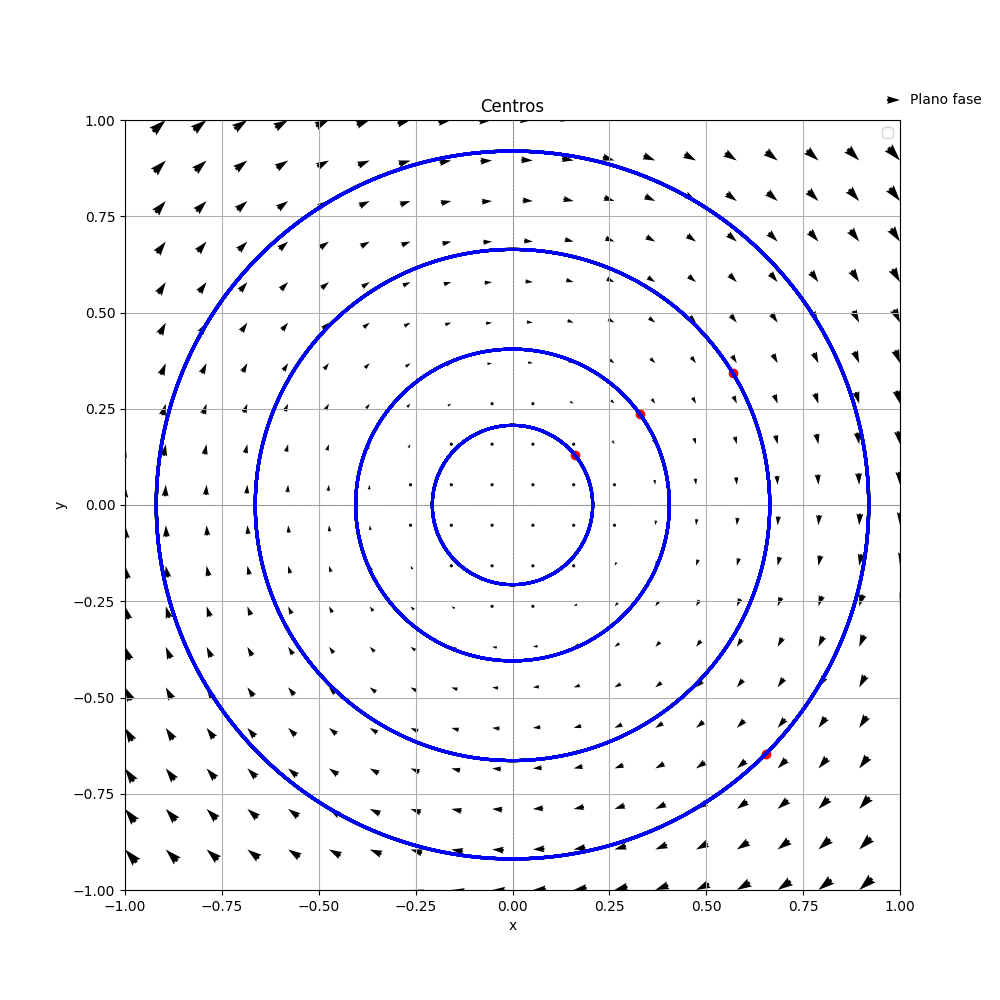
\includegraphics[width=0.7\textwidth]{Img/Centros.png}
    \caption{Centro}
    \label{fig:centro}
\end{figure}

\newpage

\subsubsection{No Aislados}

\begin{definition}
Un \textbf{equilibrio no aislado} ocurre cuando un eigenvalor es cero y el otro es distinto de cero.
\end{definition}

En este caso, las trayectorias pueden colapsar en una línea de equilibrios, lo que refleja la presencia de un subespacio invariante.

\begin{example}
Considere el sistema:
\[
\frac{d}{dt} \begin{bmatrix} x \\ y \end{bmatrix} = \begin{bmatrix} 0 & 0 \\ 0 & -1 \end{bmatrix} \begin{bmatrix} x \\ y \end{bmatrix}.
\]
Este es un \textbf{equilibrio no aislado}. Las trayectorias convergen hacia el eje $x$, que actúa como una línea de equilibrios.
\end{example}

La clasificación de puntos de equilibrio no solo nos permite entender el comportamiento local de un sistema dinámico, sino también predecir su evolución global. Cada tipo de equilibrio tiene su propia "personalidad", y su estudio revela la riqueza y complejidad de los sistemas dinámicos lineales.

\begin{figure}[h]
    \centering
    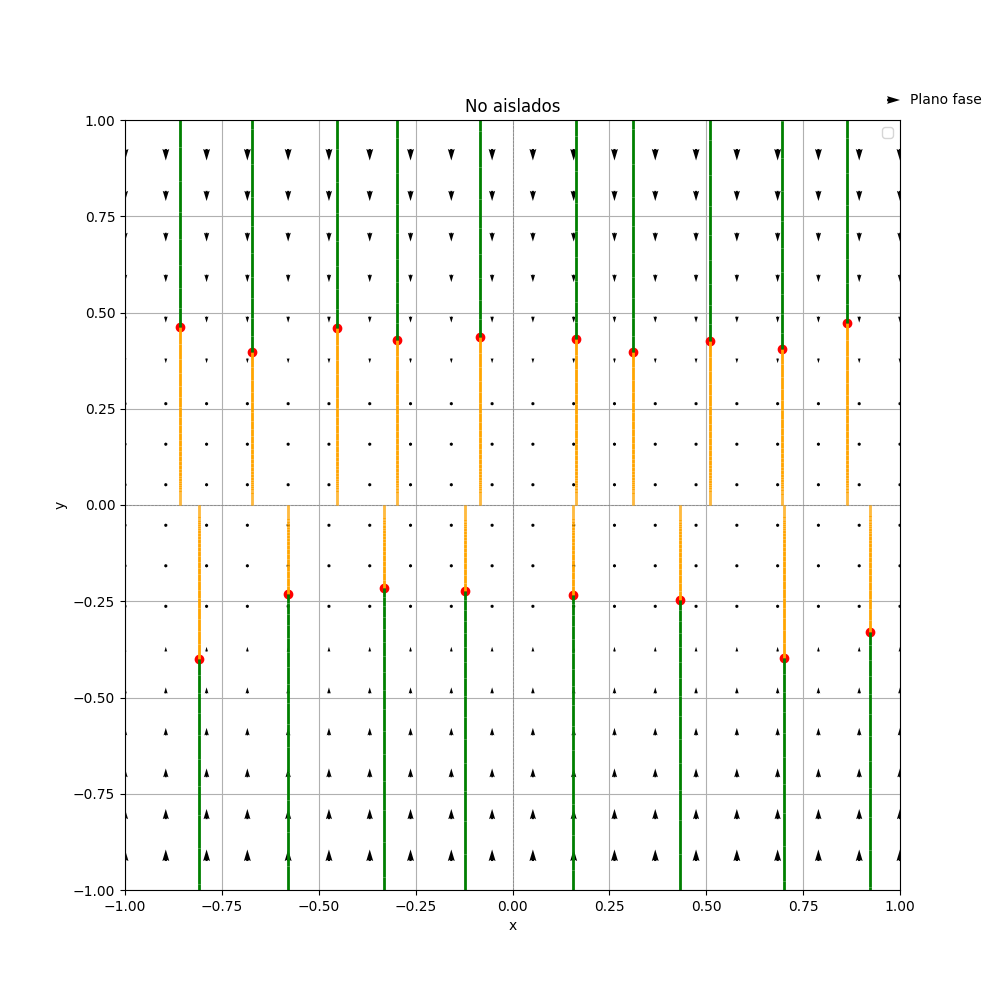
\includegraphics[width=0.7\textwidth]{Img/NoAislados.png}
    \caption{Equilibrio no aislado}
    \label{fig:no_aislado}
\end{figure}


\section{Teoría de la Linealización de Sistemas de Ecuaciones Diferenciales}

En la sección anterior, exploramos los diferentes tipos de puntos de equilibrio en sistemas lineales y su clasificación según los eigenvalores de la matriz asociada. Aprendimos cómo los nodos, puntos silla, espirales y centros describen comportamientos locales únicos, cada uno con su propia "personalidad". Sin embargo, muchos fenómenos del mundo real están modelados por sistemas no lineales, cuya complejidad puede dificultar un análisis directo. En esta sección, profundizaremos en un método clave para estudiar estos sistemas: la \textbf{linealización}.

La idea central detrás de la linealización es aprovechar las herramientas desarrolladas para sistemas lineales y aplicarlas a sistemas no lineales cerca de puntos de equilibrio. Como vimos anteriormente, los puntos de equilibrio son estados donde el sistema "se detiene", y su estabilidad determina si el sistema regresa al equilibrio o se aleja tras pequeñas perturbaciones. La linealización nos permite aproximar el comportamiento local de un sistema no lineal mediante un sistema lineal asociado, simplificando significativamente el análisis.

\subsection{De Lo Lineal a Lo No Lineal: Una Transición Natural}

Recordemos que, en sistemas lineales, el comportamiento global está completamente determinado por los eigenvalores de la matriz del sistema. Por ejemplo:
- Un \textbf{nodo estable} indica que todas las trayectorias convergen al origen.
- Un \textbf{punto silla} revela direcciones estables e inestables.
- Un \textbf{centro} describe órbitas cerradas sin convergencia ni divergencia.

Sin embargo, en sistemas no lineales, estas propiedades pueden variar dependiendo de la región del espacio fase que estemos analizando. Aquí es donde entra la linealización: al enfocarnos en un entorno pequeño alrededor de un punto de equilibrio, podemos aproximar el sistema no lineal por uno lineal que capture su comportamiento local.

\subsection{El Proceso de Linealización: ¿Cómo Funciona?}

Consideremos un sistema autónomo de ecuaciones diferenciales ordinarias (EDO) en $\mathbb{R}^n$:

\begin{equation}\label{eq:sistema_no_lineal}
    \dot{\mathbf{x}} = \mathbf{f}(\mathbf{x}),
\end{equation}

donde $\mathbf{x} \in \mathbb{R}^n$ representa el vector de estado, y $\mathbf{f}: \mathbb{R}^n \to \mathbb{R}^n$ es una función vectorial continua y diferenciable al menos una vez en un entorno del punto de equilibrio. Recordemos, como se discutió en la sección anterior, que un \textbf{punto de equilibrio} $\mathbf{x}_0$ satisface:

\begin{equation}
    \mathbf{f}(\mathbf{x}_0) = \mathbf{0}.
\end{equation}

Para analizar el comportamiento del sistema cerca de $\mathbf{x}_0$, utilizamos la \textbf{expansión en serie de Taylor} de $\mathbf{f}(\mathbf{x})$ alrededor de $\mathbf{x}_0$. Esta aproximación descompone $\mathbf{f}(\mathbf{x})$ en términos lineales y residuales:

\begin{equation}
    \mathbf{f}(\mathbf{x}) = \mathbf{f}(\mathbf{x}_0) + D\mathbf{f}(\mathbf{x}_0)(\mathbf{x} - \mathbf{x}_0) + \mathbf{R}(\mathbf{x}),
\end{equation}

donde:
- $D\mathbf{f}(\mathbf{x}_0)$ es la \textbf{matriz Jacobiana} evaluada en $\mathbf{x}_0$, cuyos elementos son $\left[ D\mathbf{f}(\mathbf{x}_0) \right]_{ij} = \dfrac{\partial f_i}{\partial x_j} \bigg|_{\mathbf{x}_0}$,
- $\mathbf{R}(\mathbf{x})$ es el término de residuo que contiene las partes de orden superior.

Como $\mathbf{f}(\mathbf{x}_0) = \mathbf{0}$, la aproximación lineal del sistema cerca de $\mathbf{x}_0$ es:

\begin{equation}\label{eq:sistema_linealizado}
    \dot{\mathbf{x}} = D\mathbf{f}(\mathbf{x}_0)(\mathbf{x} - \mathbf{x}_0).
\end{equation}

Esta ecuación describe cómo el sistema evoluciona cerca del punto de equilibrio. Es como si estuviéramos mirando el sistema a través de una lupa centrada en $\mathbf{x}_0$, ignorando los términos de orden superior que son despreciables en un entorno suficientemente pequeño.

\subsection{Eigenvalores y Estabilidad}

Al igual que en sistemas lineales, la matriz Jacobiana $D\mathbf{f}(\mathbf{x}_0)$ juega un papel crucial en la linealización. Sus eigenvalores determinan la estabilidad local del punto de equilibrio $\mathbf{x}_0$:
- Si todos los eigenvalores tienen parte real negativa ($\text{Re}(\lambda_i) < 0$), el punto de equilibrio es \textbf{asintóticamente estable}. Las trayectorias cercanas convergen al equilibrio, similar a un nodo estable.
- Si alguno de los eigenvalores tiene parte real positiva ($\text{Re}(\lambda_i) > 0$), el punto de equilibrio es \textbf{inestable}. Las trayectorias cercanas se alejan del equilibrio, como en un punto silla o un nodo inestable.
- Si todos los eigenvalores tienen parte real no positiva y al menos uno con parte real cero, el análisis lineal no es concluyente, y debemos recurrir a métodos más avanzados.

Estos resultados refuerzan lo que aprendimos en la sección anterior sobre la importancia de los eigenvalores en la clasificación de puntos de equilibrio. La diferencia clave aquí es que estamos aplicando estas ideas a sistemas no lineales, donde la linealización solo proporciona información local.

\subsection{Profundizando en la Interpretación Geométrica}

La matriz Jacobiana $D\mathbf{f}(\mathbf{x}_0)$ actúa como una "brújula" que nos indica la dirección y magnitud del cambio en cada variable del sistema cerca del punto de equilibrio. Por ejemplo:
- Si los eigenvalores tienen parte real negativa, el sistema tiende a regresar al equilibrio, como un resorte que se comprime y luego vuelve a su posición original.
- Si los eigenvalores tienen parte real positiva, el sistema se aleja del equilibrio, como una bola rodando cuesta abajo.

Este comportamiento es análogo a lo que observamos en sistemas lineales, pero ahora lo estamos aplicando a sistemas no lineales en un entorno local.

\subsection{Ejemplo Práctico: Modelo de Depredador-Presa}

Para ilustrar el proceso de linealización, consideremos nuevamente el modelo de depredador-presa discutido en la sección anterior:

\begin{equation}\label{eq:ejemplo_sistema}
    \begin{cases}
        \dot{x} = x (1 - x) - xy, \\
        \dot{y} = y (-\alpha + x),
    \end{cases}
\end{equation}

donde $x$ representa la población de presas, $y$ la población de depredadores, y $\alpha > 0$ es un parámetro que controla la tasa de crecimiento de los depredadores.

\subsubsection{Puntos de Equilibrio}

Recordemos que los puntos de equilibrio son:
\begin{itemize}
    \item $E_1 = (0, 0)$: Extinción de ambas especies.
    \item $E_2 = (1, 0)$: Las presas alcanzan su capacidad máxima sin depredadores.
    \item $E_3 = (\alpha, 0)$ si $0 < \alpha < 1$: Coexistencia de presas y depredadores.
\end{itemize}

\subsubsection{Linealización en $E_2 = (1, 0)$}

Calculamos la matriz Jacobiana:

\begin{equation}
    \mathbf{A} = D\mathbf{f}(x, y) =
    \begin{pmatrix}
        1 - 2x - y & -x \\
        y & -\alpha + x
    \end{pmatrix}.
\end{equation}

Evaluamos en $E_2 = (1, 0)$:

\begin{equation}
    \mathbf{A}|_{(1,0)} =
    \begin{pmatrix}
        -1 & -1 \\
        0 & 1 - \alpha
    \end{pmatrix}.
\end{equation}

Los eigenvalores son las soluciones de:

\begin{equation}
    \det(\mathbf{A} - \lambda \mathbf{I}) = 0.
\end{equation}

Resolviendo, obtenemos:

\begin{equation}
    \lambda_1 = -1, \quad \lambda_2 = 1 - \alpha.
\end{equation}

La estabilidad del punto de equilibrio $E_2$ depende del valor de $\alpha$:
- Si $\alpha < 1$, entonces $\lambda_2 > 0$, y el punto es un \textbf{punto silla} (inestable). Las perturbaciones pueden llevar al sistema hacia otros estados.
- Si $\alpha > 1$, entonces $\lambda_2 < 0$, y el punto es un \textbf{nodo estable}. El sistema tiende a regresar al equilibrio.

Este análisis refuerza lo que aprendimos en la sección anterior sobre la importancia de los puntos silla y nodos en la dinámica de sistemas.

La linealización es una herramienta poderosa que conecta los conceptos de puntos de equilibrio y estabilidad de sistemas lineales con el análisis de sistemas no lineales. Al aproximar el comportamiento local de un sistema no lineal mediante su linealización, podemos aplicar las mismas herramientas y técnicas que usamos en la sección anterior, como la clasificación de puntos de equilibrio basada en eigenvalores.

Este enfoque no solo simplifica el análisis, sino que también brinda intuiciones valiosas sobre cómo interactúan las variables en sistemas complejos. Desde modelos ecológicos hasta sistemas mecánicos, la linealización sigue siendo una piedra angular en el estudio de sistemas dinámicos, permitiéndonos comprender tanto el comportamiento local como sus implicaciones globales.

